We now evaluate the performance of our word embedding compression algorithm on a variety of NLP tasks and embeddings types.
We show that our compression method is consistently able to match the performance of more complex baselines (DCCL, k-means), while dramatically outperforming more naive baselines (dimensionality reduction).
We additionally present results in which we maintain the memory budget fixed by  jointly varying the dimension and precision of the compressed embeddings;
we observe that in this memory-constrained setting, the best compressed embeddings attain \todo{XX\%} to \todo{YY\%} better performance than the full-precision embeddings.
This demonstrates the importance of considering low-precision when trying to attain the best possible performance under a memory budget.

\subsection{Large-scale evaluation}
\begin{itemize}
	\item \textbf{Embeddings}: GloVe ($d\in\{50,100,200,300\}$, $n=400k$) and fastText ($d=300$, $n=10^6$) pre-trained.
	\item \textbf{Baselines}: k-means, DCCL, dim. reduction (GloVe)
	\item \textbf{Tasks}: DrQA, sentiment, intrinsics, synthetics.
	\item \textbf{Compression ratios}: 8x-32x.
	\item \textbf{Number of random seeds}: 5
\end{itemize}

In Figure~\ref{fig:glove400k_drqa} we show that our uniform quantization method performs comparably to k-means and DCCL, while performing significantly better than the dimensionality reduction baseline.

%\begin{figure}
%\begin{center}
%\centerline{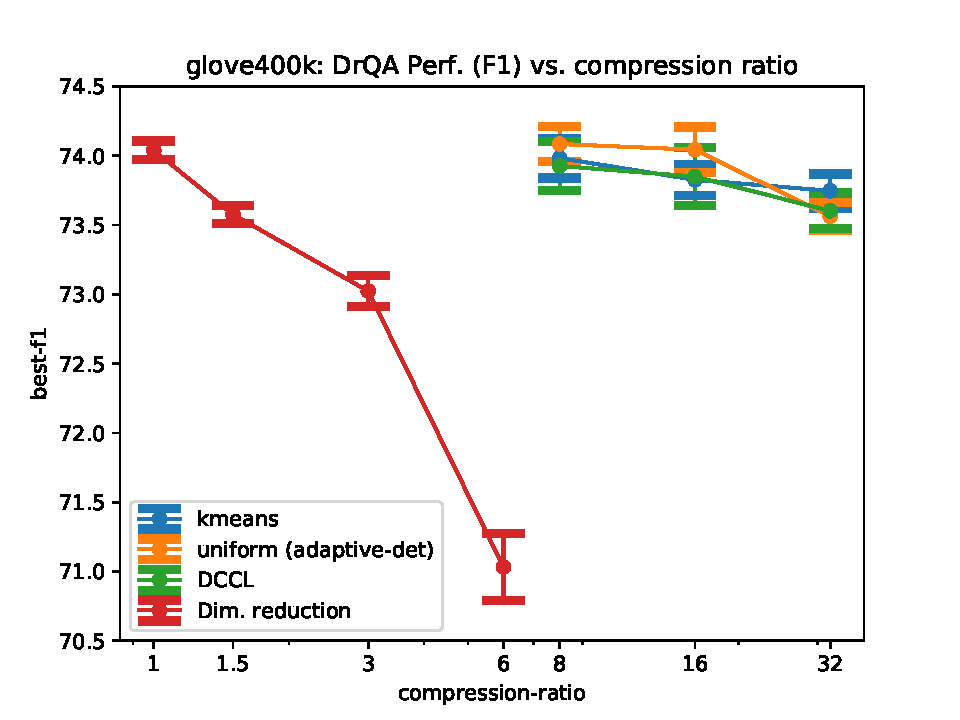
\includegraphics[width=\columnwidth]{figures/glove400k_drqa_vs_compression.pdf}}
%\caption{Question answering performance (DrQA) for a number of compression methods at various compression ratios, on pre-trained GloVe embedding.  Uniform quantization performs similarly to k-means and DCCL, while significantly outperforming the dimensionality reduction baseline. \todo{TODO: Include fastText results (though there won't be a dim. reduction baseline, since they don't release pre-trained embeddings at smaller dimensions.)}}
%\label{fig:glove400k_drqa}
%\end{center}
%\end{figure}




\begin{figure*}
	\centering
	\begin{small}
		%		\begin{tabular}{c c c c}
		\begin{tabular}{@{\hskip -0.0in}c@{\hskip -0.0in}c@{\hskip -0.0in}}
			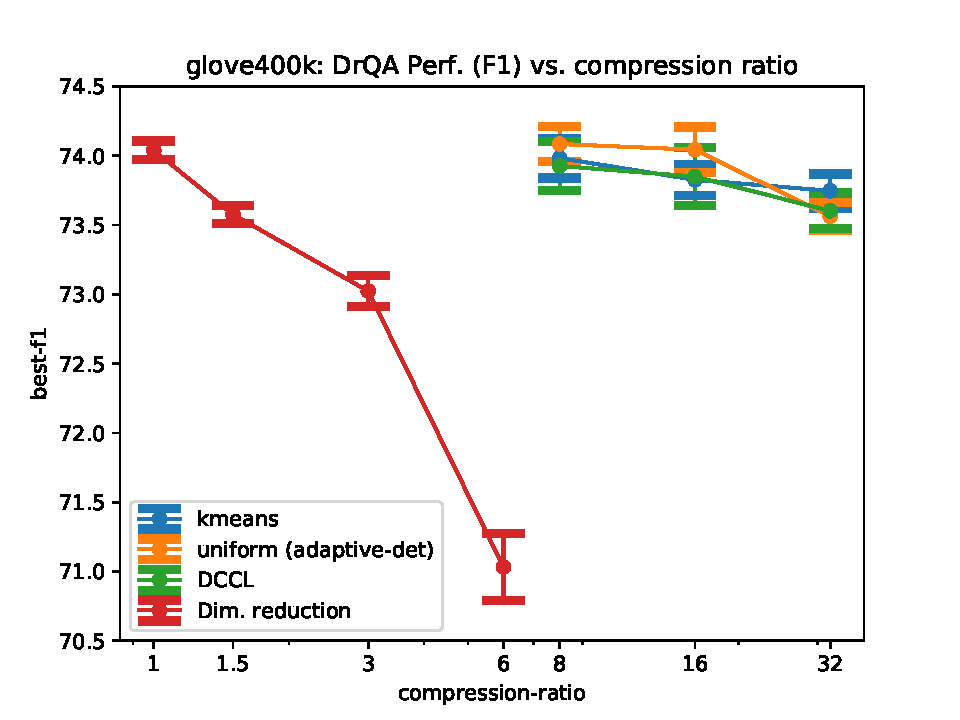
\includegraphics[width=0.45\linewidth]{figures/glove400k_drqa_vs_compression.pdf} &
			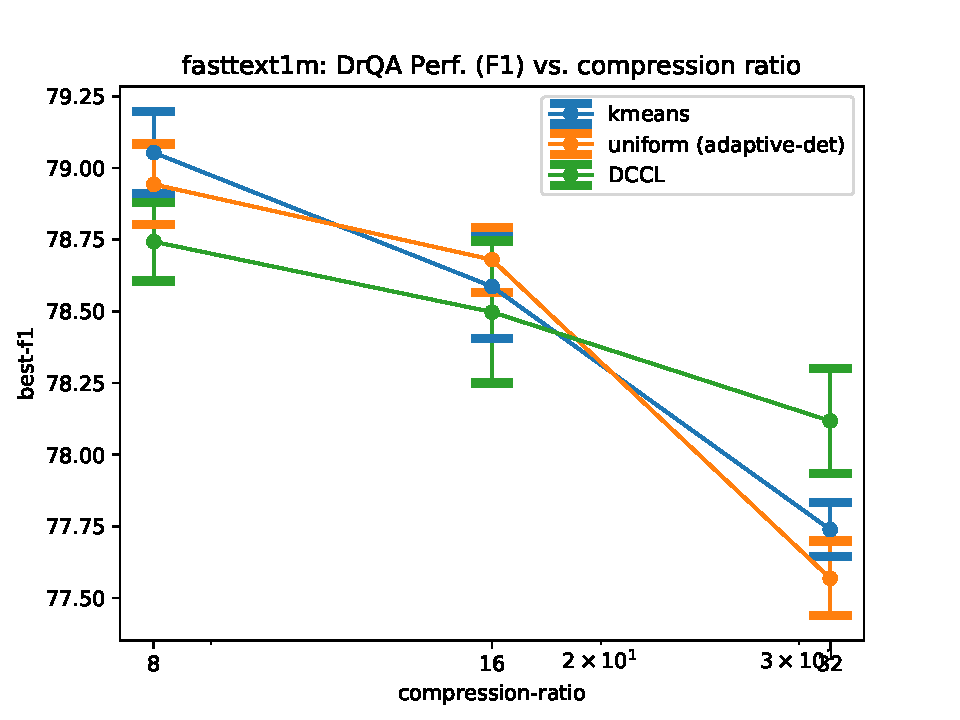
\includegraphics[width=0.45\linewidth]{figures/fasttext1m_drqa_vs_compression.pdf} \\
			\;\;\;\;\;(a) & \;\;\;\;\;\;(b) 
		\end{tabular}
	\end{small}
\caption{Question answering performance (DrQA) for a number of compression methods at various compression ratios, on pre-trained 300-dimensional GloVe and fastText embeddings.  Uniform quantization performs similarly to k-means and DCCL.  For GloVe, we are also able to compare with pre-trained embeddings of smaller dimensions ($d\in\{50,100,200,300\}$), and observe that compressing the 300-dimensional embeddings is significantly better than using a lower dimension.}
\label{fig:glove400k_drqa}
\end{figure*}



\subsection{Fixed budget experiments}
\begin{itemize}
	\item \textbf{Embeddings}: We train GloVe embeddings on a Wiki 2017 dump, for $n=400k$ and $d \in \{25,50,100,200,400,800\}$.
	\item \textbf{Bitrates}: We compress embeddings for $b \in \{1,2,4,8,16,32\}$.
	\item \textbf{Tasks}: DrQA, sentiment, intrinsics, synthetics.
	\item \textbf{Number of random seeds}: 5
\end{itemize}

In Figure~\ref{fig:glove400k_dim_vs_prec}, we show that when considering a fixed memory budget, it is best to use low-precision and high-dimensions.

\begin{figure}
	\begin{center}
		\centerline{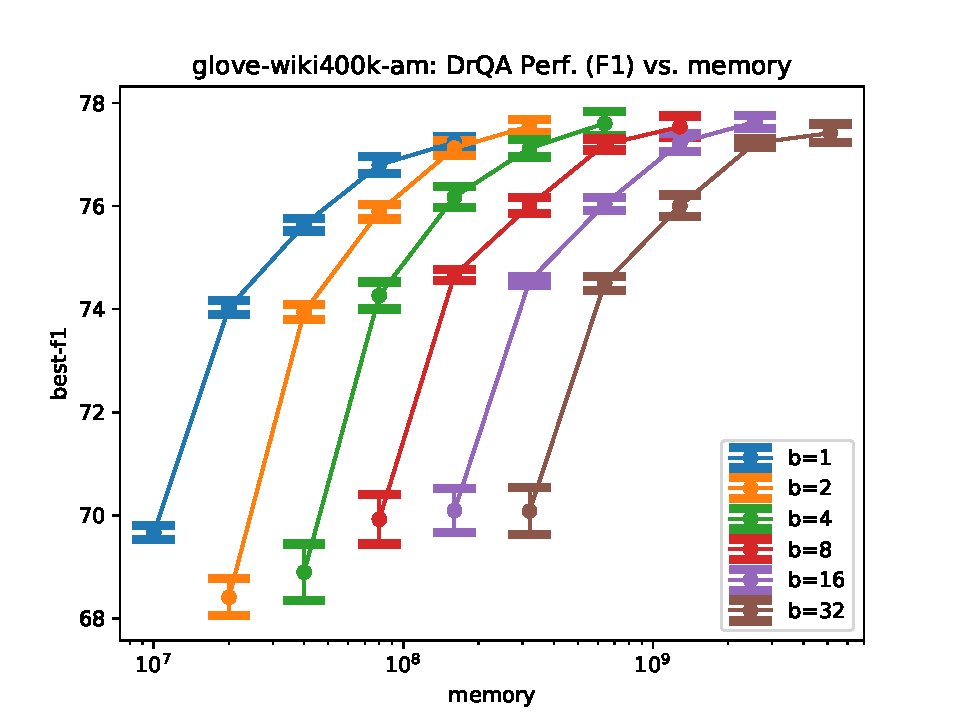
\includegraphics[width=\columnwidth]{figures/glove-wiki400k-am_drqa_vs_compression.pdf}}
		\caption{We compress GloVe embeddings for dimensions $d\in\{25,50,100,200,400\}$ at precision values $b\in\{1,2,4,8,16,32\}$, and measure performance on question-answering (DrQA).  \todo{TODO: Include $d=800$ results, which are worse than $d=400$?}}
		\label{fig:glove400k_dim_vs_prec}
	\end{center}
\end{figure}
